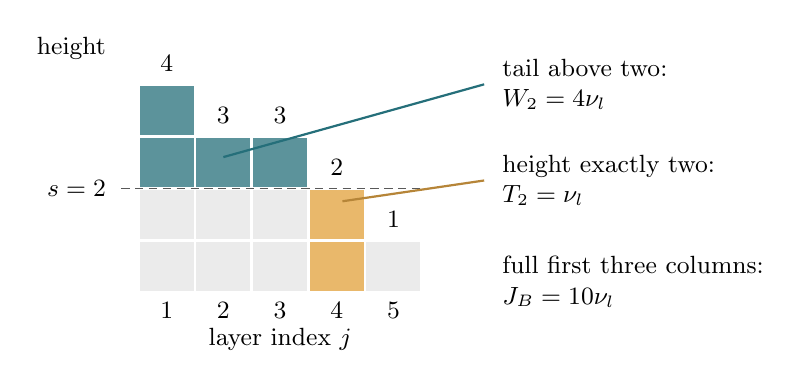
\begin{tikzpicture}[x=0.72cm,y=0.66cm,font=\small]
 \definecolor{layertail}{RGB}{37,111,122}
 \definecolor{layertwo}{RGB}{227,166,70}
 \foreach \j/\height in {1/4,2/3,3/3,4/2,5/1} {
  \foreach \i in {1,...,\height} {
   \fill[black!8] (\j-1,\i-1) rectangle (\j,\i);
   \ifnum\i>2
    \fill[layertail!75] (\j-1,\i-1) rectangle (\j,\i);
   \fi
   \ifnum\j=4
    \fill[layertwo!80] (\j-1,\i-1) rectangle (\j,\i);
   \fi
   \draw[white,line width=1pt] (\j-1,\i-1) rectangle (\j,\i);
  }
  \node[below] at (\j-0.5,0) {\(\j\)};
  \node[above] at (\j-0.5,\height+0.05) {\(\height\)};
 }
 \draw[densely dashed,black!65] (-0.3,2)--(5.3,2);
 \node[anchor=east] at (-0.4,2) {\(s=2\)};
 \node[anchor=east] at (-0.4,4.7) {height};
 \node at (2.5,-0.9) {layer index \(j\)};
 \draw[layertail,thick] (1.5,2.6)--(6.1,4.0);
 \node[anchor=west,align=left] at (6.25,4.0)
   {tail above two:\\ \(W_2=4\nu_l\)};
 \draw[layertwo!80!black,thick] (3.6,1.75)--(6.1,2.15);
 \node[anchor=west,align=left] at (6.25,2.15)
   {height exactly two:\\ \(T_2=\nu_l\)};
 \node[anchor=west,align=left] at (6.25,0.2)
   {full first three columns:\\ \(J_B=10\nu_l\)};
\end{tikzpicture}
